\documentclass[a4paper,12pt,oneside,final]{report}
\usepackage[pdftex]{graphicx}
\usepackage{amssymb}
\usepackage{epstopdf}
\usepackage[utf8]{inputenc}
\usepackage{titlesec}
\usepackage[titletoc]{appendix}
\titleformat{\chapter}[hang]{\bf\Huge}{\thechapter}{1cm}{}

\usepackage[colorlinks=true]{hyperref}
\hypersetup{urlcolor=blue,linkcolor=black,citecolor=black,colorlinks=true}
\bibliographystyle{plain}

\pagestyle{plain}
% -------------------- this stuff for code --------------------

\usepackage{anysize}
\marginsize{30mm}{30mm}{20mm}{20mm}

\newenvironment{formal}{%
  \def\FrameCommand{%
    \hspace{1pt}%
    {\color{blue}\vrule width 2pt}%
    {\color{formalshade}\vrule width 4pt}%
    \colorbox{formalshade}%
  }%
  \MakeFramed{\advance\hsize-\width\FrameRestore}%
  \noindent\hspace{-4.55pt}% disable indenting first paragraph
  \begin{adjustwidth}{}{7pt}%
  \vspace{2pt}\vspace{2pt}%
}
{%
  \vspace{2pt}\end{adjustwidth}\endMakeFramed%
}

\newenvironment{changemargin}[2]{\begin{list}{}{%
\setlength{\topsep}{0pt}%
\setlength{\leftmargin}{0pt}%
\setlength{\rightmargin}{0pt}%
\setlength{\listparindent}{\parindent}%
\setlength{\itemindent}{\parindent}%
\setlength{\parsep}{0pt plus 1pt}%
\addtolength{\leftmargin}{#1}%
\addtolength{\rightmargin}{#2}%
}\item }{\end{list}}

\usepackage{color}
\usepackage{dsfont}
\usepackage[bitstream-charter]{mathdesign}
\usepackage[scaled]{helvet}
\usepackage{inconsolata}

\usepackage[usenames,dvipsnames]{xcolor}

\definecolor{colKeys}{rgb}{0,0,0.9} 
\definecolor{colIdentifier}{rgb}{0,0,0} 
\definecolor{colString}{rgb}{0.7,0,0} 
\definecolor{colComments}{rgb}{0,0.6,0} 
\usepackage{listings}
\lstset{
  stringstyle=\color{colString},
  keywordstyle=\color{colKeys},
  identifierstyle=\color{colIdentifier},
  commentstyle=\color{colComments},
  numbers=left,
  tabsize=4,
  frame=single,
  breaklines=true,
  basicstyle=\small\ttfamily,
  numberstyle=\tiny\ttfamily,
  framexleftmargin=0mm,
  xleftmargin=7mm,
  xrightmargin=7mm,
  frameround={tttt},
  captionpos=b
}

\usepackage{mathtools}
\usepackage{amsthm}
\newtheorem{definition}{Definition}
\newtheorem{theorem}{Theorem}
\DeclareMathOperator*{\argmin}{ArgMin\ }
\DeclareMathOperator*{\argmax}{ArgMax\ }

\usepackage{algorithm}
\usepackage{algorithmic}

\makeatletter
\DeclareRobustCommand{\em}{%
  \@nomath\em \if b\expandafter\@car\f@series\@nil
  \normalfont \else \bfseries \fi}
\makeatother

%% Headers and footers
\usepackage{fancyhdr}
\usepackage[section]{placeins}
\pagestyle{fancy}
\fancyhf{}
\addtolength{\headwidth}{30pt}
\addtolength{\headwidth}{30pt}
\renewcommand{\headrulewidth}{0.4pt} % thickness of the header line
\renewcommand{\footrulewidth}{0.4pt} % thickness of the footer line
\renewcommand{\chaptermark}[1]{\markboth{#1}{#1}} % chapter name
\renewcommand{\sectionmark}[1]{\markright{\thesection\ #1}}  % section name
\lhead[\fancyplain{}{\bf\thepage}]{\fancyplain{}{\bf\rightmark}} % display header
\rhead[\fancyplain{}{\bf\leftmark}]{\fancyplain{}{}} % display header
\fancyfoot[C]{\bf\thepage} % display footer (page number)
\fancyfoot[R]{\bf\today} % display footer (date)
\fancypagestyle{plain}{ 
	\fancyhead{} \renewcommand{\headrulewidth}{0pt}
}
\newcommand{\clearemptydoublepage}{\newpage{\pagestyle{plain}\cleardoublepage}}

\usepackage[T1]{fontenc}
\usepackage{enumerate}
\usepackage{afterpage,lastpage,fancyhdr}
\usepackage[includeheadfoot,margin=2.5cm]{geometry}
\geometry{letterpaper}                   % ... or a4paper or a5paper or ... 

\DeclareGraphicsRule{.tif}{png}{.png}{`convert #1 `dirname #1`/`basename #1 .tif`.png}

\makeatletter \def\thickhrulefill{\leavevmode \leaders \hrule height 1pt\hfill
\kern \z@} \renewcommand{\maketitle}{
    \begin{titlepage}
    \let\footnotesize\small \let\footnoterule\relax \parindent \z@ \reset@font
    \null\vfil
    \vspace{-20mm}
    \begin{center}
    {\small \scshape Imperial College London \\ Department of Computing}
    \end{center}
    \vspace{0.5cm}
	\begin{minipage}{\textwidth}
		\vspace{1cm}
		\noindent\rule[0ex]{\textwidth}{4pt} \\
		\flushright
		\center
		\@title
		\\ \vspace{4mm}
		\noindent\rule[0ex]{\textwidth}{4pt} \\
	\end{minipage}
	\vspace{1.5cm}
	\begin{minipage}{\textwidth}
		\flushright
		{\bfseries}
		\vspace{7mm}
		\flushleft
		\@author.\\
	\end{minipage}
	\vspace{0.5cm}
	\begin{center}
		
\includegraphics[width=70mm,]{pictures/logo_imperial_college_london.png}
	\end{center}
	\vspace{\stretch{1}}
	\vspace{50mm}
		\flushleft
		{\bfseries}
		Module leader \& Lecturer: Dr Abhijeet \textsc{Ghosh}. \\
		{\small \scshape \@date }.
		\vspace{0.1cm}
		\rule{\linewidth}{.5pt}
  \end{titlepage}
  \setcounter{footnote}{1}
  \setcounter{page}{2}
}


\author{
	Jean \textsc{Kossaifi} (jk712)\\
    Romain \textsc{Brault} (rb812)\\
}
\makeatother
\title{\Huge C417: Advanced Graphics \\ Coursework 1}
\date{\today}


\usepackage{amsmath}
\begin{document}
\maketitle
\tableofcontents

\chapter{Introduction}
\paragraph{}
The aim of this coursework is to implement to simple algorithm. The first one assemble an HDR image and tone map the result so it can be rendered on a screen. The second algorithm map a latitude longitude map on a sphere.
\paragraph{}
To obtain the maximum throughput we have followed the advices proposed by Intel \cite{Petter2009intel} to represent an image. The idea is to represent an image as blocks of 8 pixelsn with continuous red green and blue pixels chanel. This representation allows the compiler to vectorise the code of some loops, allowing them do compute multiple values at the same time. Of course writing and reading images on the hard drive takes more time, however we the improvement during the HDR assembly or the sphere mapping compensate this overhead.
\paragraph{}
\begin{table}[htbp]
\centering
\begin{tabular}{|c|c|c|c|c|c|c|c|c|c|c|c|}
\hline
$R_1$ & $G_1$ & $B_1$ & $R_2$ & $G_2$ & $B_2$ & $R_3$ & $G_3$ & $B_3$ & $R_4$ & $G_4$ & $B_4$ \\ \hline
$R_5$ & $G_5$ & $B_6$ & $R_6$ & $G_6$ & $B_6$ & $R_7$ & $G_7$ & $B_7$ & $R_8$ & $G_8$ & $B_8$ \\
\hline
\end{tabular}
\caption{Classic image representation.}
\end{table}
\begin{table}[htbp]
\centering
\begin{tabular}{|c|c|c|c|c|c|c|c|c|c|c|c|}
\hline
$R_1$ & $R_2$ & $R_3$ & $R_4$ & $R_5$ & $R_6$ & $R_7$ & $R_8$ & $G_1$ & $G_2$ & $G_3$ & $G_4$ \\ \hline
$G_5$ & $G_6$ & $G_7$ & $G_8$ & $B_1$ & $B_2$ & $B_3$ & $B_4$ & $B_5$ & $B_6$ & $B_7$ & $B_8$ \\
\hline
\end{tabular}
\caption{Vectorised image representation.}
\end{table}
\paragraph{}
We have also slightly alter the proposed algorithm to obtain better visual results. Theses modifications are local and do not change the general flow of the algorithms. They are all explained below.
\paragraph{}
We have choosen to do this coursework in C++ since this language allows us to use some high level tools and simplify the developpement but is also a language widely use for High Performance Computing and Computer Vision. We also used the Qt libray to build a simple GUI and OPenMP to parallelise the computations. The binaries \textit{HDRimage} and \textit{relightning} should be compatible on every x86\_64 linux machine (we tried them in the lab and on our personal computer). To use them:
\begin{itemize}
\item clic on \textit{Files} then \text{Open} and select all the memorial images;
\item if necessary, adjust the coefficients and clic on \textit{Set Coefs};
\item clic on \textit{Create HDR};
\item adjust the Stops and Gamma with the sliders;
\item clic on \textit{Files} then \textit{Save} to save the image as a \textit{.pfm} or \textit{.ppm}. The \textit{.pfm} file is saved as the raw HDR image, whereas the \textit{.ppm} file is saved after the tone mapping and gamma correction.
\end{itemize}

\begin{figure}[!h]
\centering
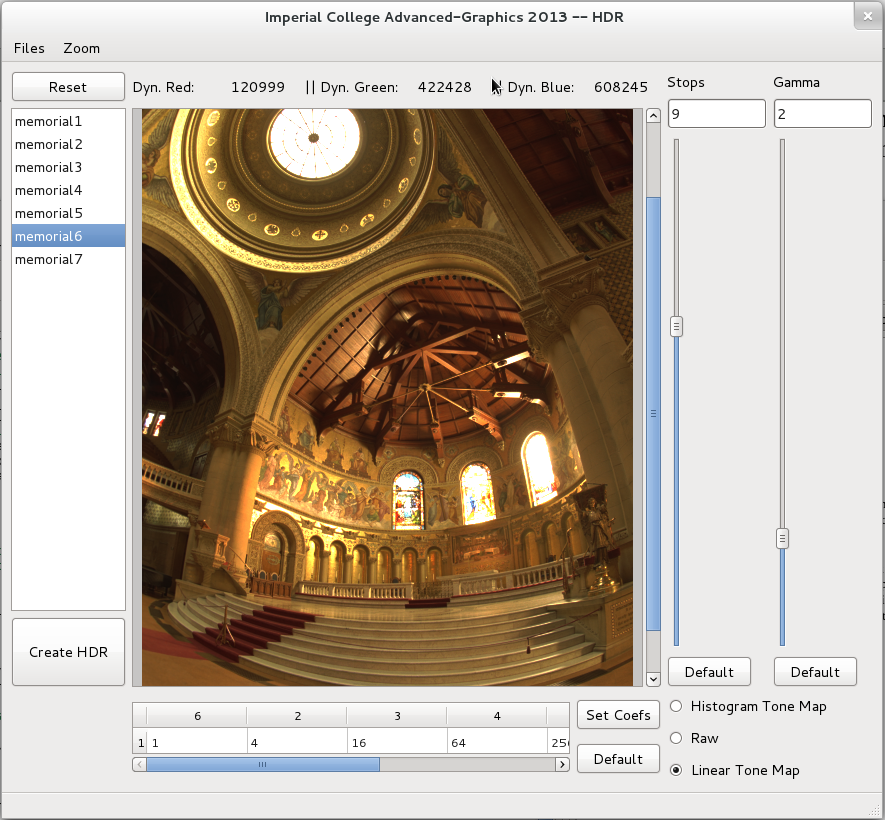
\includegraphics[height=\textheight/2]{pictures/gui.png}
\caption{GUI for HDR assembly.}
\end{figure}


\chapter{Assemble an HDR Image}
\section{Algorithm}
\paragraph{}
We first followed the instruction proposed by the coursework and the publication of Debevec \& Malik \cite{debevec2008recovering}. We used the following polynom: $w(x)=16x^2(x-1)^2$. We have $w(0)=0,\ w(1)=0,\ w(0.5)=1$ and $w'(x)=32x(2x^2-3x+1)$ thus $w'(0)=0$ and $w'(1)=0$. We have choosen a polynom rather than a trigonometric function because a polynom is faster to compute.
\begin{figure}[!h]
\centering
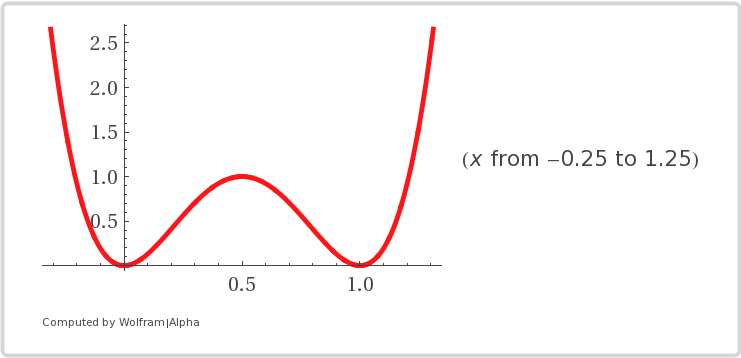
\includegraphics[width=\textwidth]{pictures/curve.png}
\caption{Polynomial curve used for the HDR weightening}
\end{figure}


\paragraph{}
However the result were not as good as expected. We noticed mutiple chromatic artifacts, circled in red on Figure \ref{img:res_raw}.
\begin{figure}[!h]
\centering
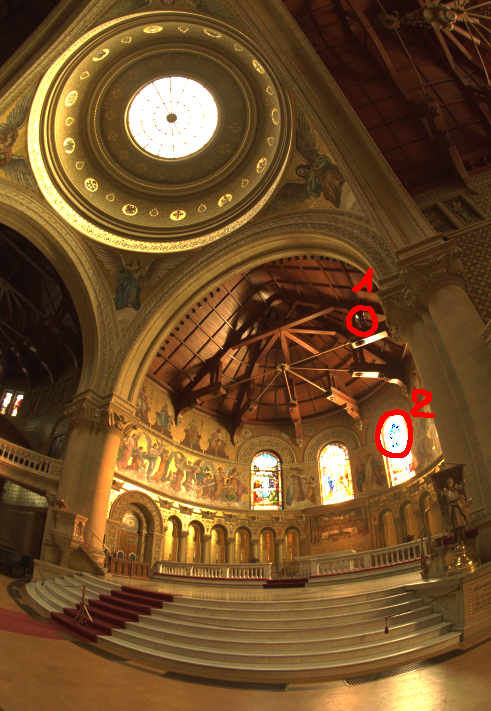
\includegraphics[scale=0.8]{pictures/raw_res.png}
\caption{First result, stops = $9$, gamma=$2$}
\label{img:res_raw}
\end{figure}
\cleardoublepage
\paragraph{}
One can notice a bunch of blue points on the window (2) which should be white, and two blue points on the wood which should be brown. The blue artifacts on the window are due to an indeterminate value of the exponential. Some pixels are so bright that they are ignored on each base picture. Thus the total sum of weight is null and the value of the fraction $\frac{\sum_ilog(E_i(x,y))w(Z_i(x,y))}{\sum_iw(Z_i(x,y))}$ undeterminate. We have opted for the following solution: each time a pixel is ignored, we change the value of a \textit{balance} variable. We increase it by one if we are over $0.92$ and decrease it by one if we are under $0.005$. After having scan all the images for a pixel (x,y) we replace the pixel value by $1$ if the balance is positive and $0$ if the balance is negative. If the balance is $0$ then we do the normal computation: $F(x,y)=exp\left(\frac{\sum_ilog(E_i(x,y))w(Z_i(x,y))}{\sum_iw(Z_i(x,y))}\right)$. We obtained the following result:
\begin{figure}[!h]
\centering
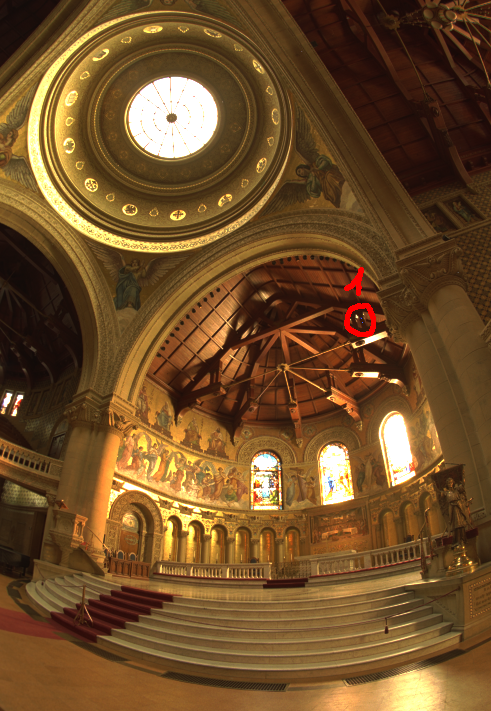
\includegraphics[scale=0.5]{pictures/raw2_res.png}
\caption{Second result, stops = $9$, gamma=$2$}
\label{img:res_raw2}
\end{figure}
\cleardoublepage
\paragraph{}
We can see on Figure \ref{img:res_raw2} that the blue artifacts on the window have been removed. However we can still see the two blue points on the wood. We analysed the seven given pictures and noticed that this blue points were due to two white points on the memorial 2 ($\Delta_t=2$).
\begin{figure}[!h]
\centering
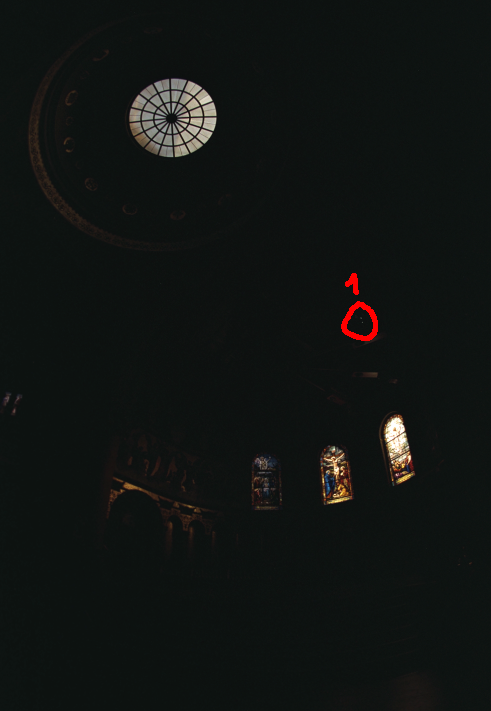
\includegraphics[scale=0.5]{pictures/memorial2.png}
\caption{Memorial $\Delta_t=2$}
\end{figure}
\cleardoublepage
This points should not be white and are probably caused by a defect of the camera. Indeed, when the exposure time $\Delta_t$ increase, the luminosity of a pixel should only increase since we are trying to find a constant radiance value. Hence we have decided to also ignore a pixel if its luminosity on picture $l$, with exposure $\Delta_t$ is over its luminosity on picture $l+1$ with an exposure of $\Delta_{t+1}>\Delta_t$.
\section{Final results}
\paragraph{}
We found the following dynamic range on each color chanel:
\begin{itemize}
\item {\bf red:} $1,20999*10^5$;
\item {\bf blue:} $4.22428*10^5$;
\item {\bf green:} $6.08245*10^5$;
\end{itemize}
\paragraph{}
Of course stops=$0$ means that we tone map from $[0;1]\subset\mathbb{R}\to[0;255]\subset\mathbb{N}$, thus no exposure function has been applyed. Simillary, if gamma=$1$, no gamma correction has been applyed. In this report only the base and the best looking pictures are presented. The others are availables in the folder "\textit{Results/part1/ppm}".
\begin{figure}[!h]
\centering
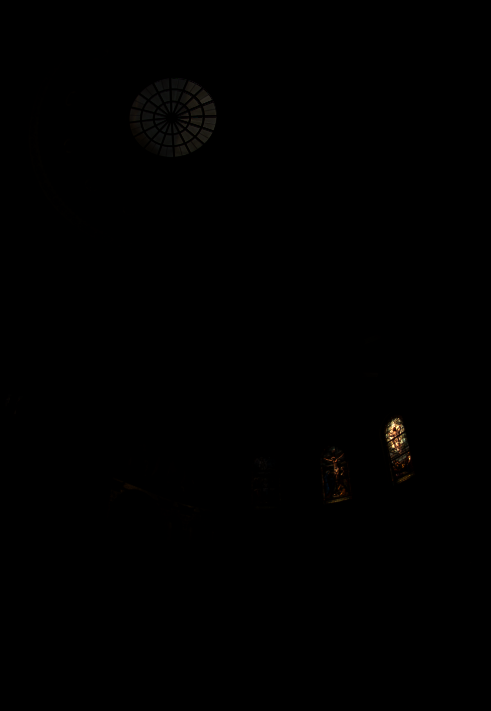
\includegraphics[scale=0.8]{pictures/stops_0_gamma_1.png}
\caption{Memorial stops=$0$, gamma=$1$. This is the image with the simplest tone map function.}
\end{figure}
\begin{figure}[!h]
\centering
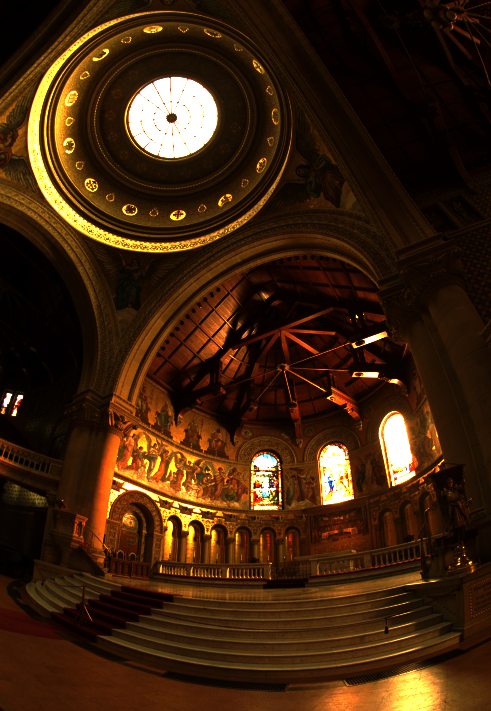
\includegraphics[scale=0.8]{pictures/stops_9_gamma_1.png}
\caption{Memorial stops=$9$, gamma=$1$. This is the best stops parameter.}
\end{figure}

\begin{figure}[!h]
\centering
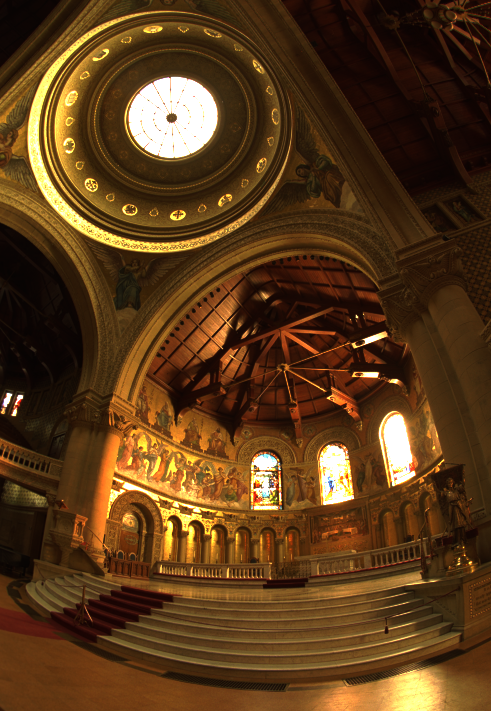
\includegraphics[scale=0.8]{pictures/stops_9_gamma_15.png}
\caption{Memorial stops=$9$, gamma=$1.5$. This is the best looking picture we found.}
\end{figure}

\begin{figure}[!h]
\centering
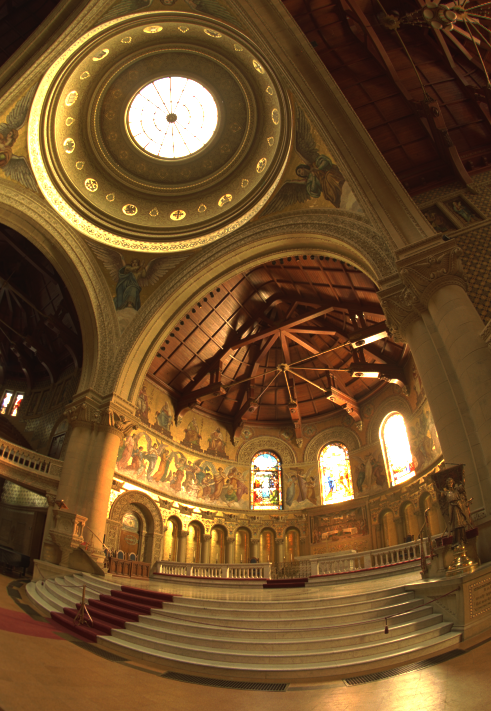
\includegraphics[scale=0.8]{pictures/stops_9_gamma_2.png}
\caption{Memorial stops=$9$, gamma=$2$. Here gamma is too large, colors are flatten.}
\end{figure}

\begin{figure}[!h]
\centering
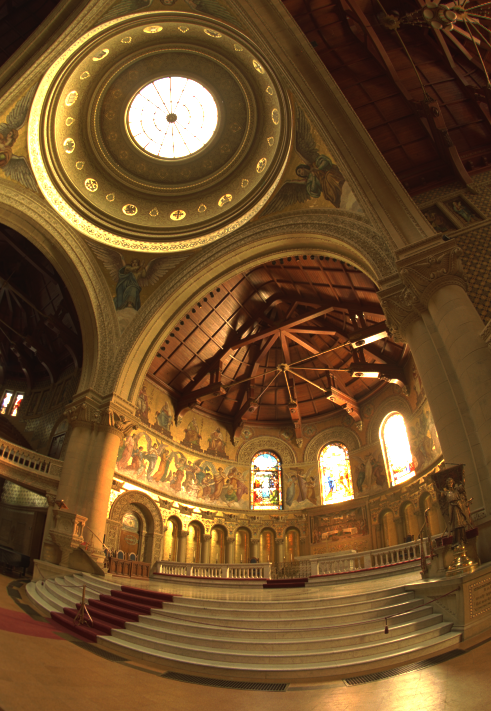
\includegraphics[scale=0.7]{pictures/stops_9_gamma_2.png}
\caption{Memorial stops=$9$, gamma=$2$. Here we tried with a new function $w(x)=sin(2\pi x-\frac{\pi}{2})+1$. We can see no differences with bare eyes from the picture generated with the polynom. The new dynamic range is red=$1,20931*10^5$, green=$6.08245*10^5$, blue=$4.22428*10^5$. With 6 digit precision, only the dynamic range of the red chanel have changed, showing that de difference between those two function is slight.}
\end{figure}

\begin{figure}[!h]
\centering
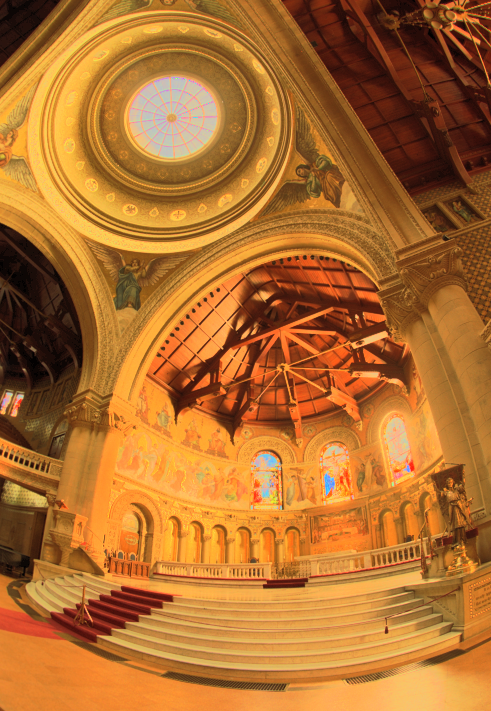
\includegraphics[scale=0.7]{pictures/hist_stops_-063_gamma_164.png}
\caption{Memorial stops=$-0.63$, gamma=$1.64$. We tried another tone map based  on an histogram expansion on grey value. The image looks less realistic (colors are not preserved) however we can see more details on the windows. The purple colors at the top of the image seems to be some artifacts due to the saturation of the pixel luminosity. Maybe a local histogram equalisation would have lead to better results.}
\end{figure}

\begin{figure}[!h]
\centering
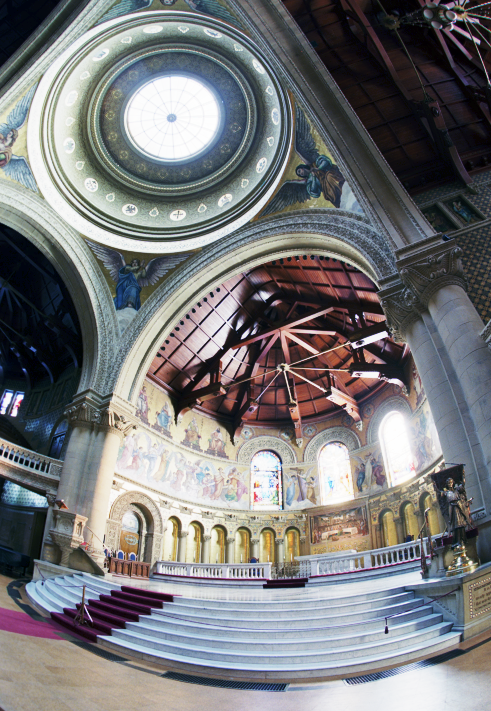
\includegraphics[scale=0.7]{pictures/dummy.png}
\caption{Memorial stops=$0$, gamma=$1$. Eventually we tried an histogram equalisation independently on each chanel. The results seems more natural but the colors are not preserved. This feature has been removed from the program since this tone map does not preserve the colors.}
\end{figure}

\chapter{Simple Image Based Lighting}
\section{Reflection sphere}
\begin{figure}[!h]
\centering
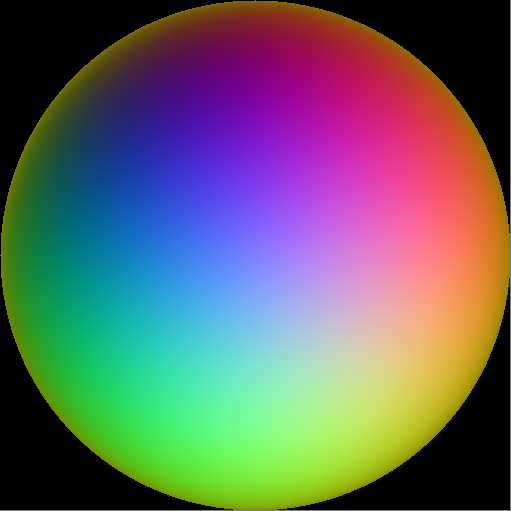
\includegraphics[scale=0.7]{pictures/reflection_sphere.png}
\caption{Reflection sphere for $v=(0,0,1)$, reflectivity = 1.}
\end{figure}

\section{Final results}
\begin{figure}[!h]
\centering
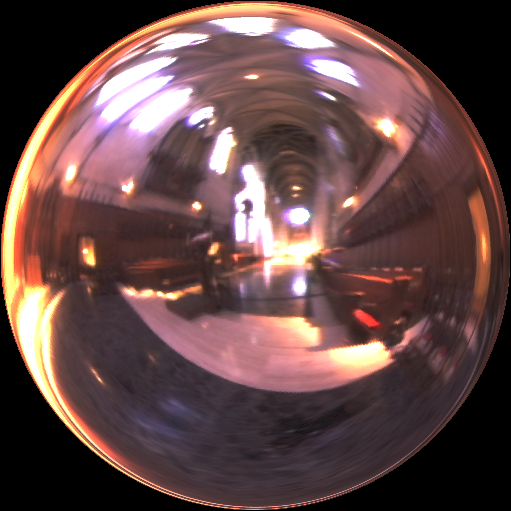
\includegraphics[scale=0.9]{pictures/final.png}
\caption{Latlong mapped on the sphere.}
\end{figure}

\begin{figure}[!h]
\centering
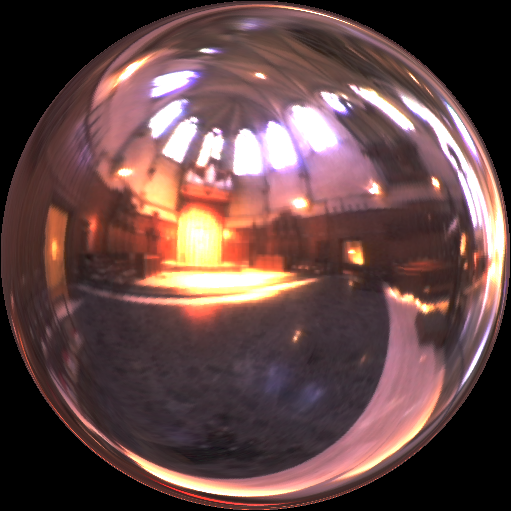
\includegraphics[scale=0.9]{pictures/final_rotate3.png}
\caption{Latlong mapped on the sphere. We can add a rotation effect by applying an offset on the $\phi$ axis.}
\end{figure}

\bibliographystyle{IEEE}
\bibliography{biblio.bib}

\end{document}